\chapter{系统设计与实现}
本章根据企业的的痛点需求,设计并实现了一个气井智能管控系统,系统包含了第三章的
结合RFM与核密度估计的气井分类算法和第四章的基于transformer的气井产量预测算法及开关井推荐。
主要包括数据连接,对连接后的油气田数据进行数据管理,对油气田数据进行可视化展示,对油气田数据
进行智能分析以及用户和权限管理等功能。
\section{系统需求分析}
\subsection{总体需求分析}
当今,陕西某油田企业作为气井行业的重要参与者,面临着诸多数字化建设方面的挑战。随着气井数量的增多以及老井的管理难度加大,需要按照气井全生命周期管理理念,引入机器学习、大数据分析、认知计算等前沿技术,提升气井及生产管理的研究决策质量和效率。

首先,过去企业由于缺乏对数据的智能分析,常常只能依赖经验进行盲目的决策。这种情况下,无法充分利用数据来指导决策,导致了生产计划不稳定,资源利用效率低下等问题。同时,对数据的分析的缺乏,使得企业难以及时发现和处理气井的异常情况,增加了生产风险和成本。

其次,该油田企业的软件应用呈现出分散使用的现象。由于业务的多样性和复杂性,企业内部采用了多种不同的软件来支持各类业务操作,这些软件可能是由不同的供应商开发的,各自为不同的业务平台提供服务。这种情况下,不同软件之间的信息流动受到限制,数据难以在不同平台之间实现无缝对接与共享,导致了信息孤岛的形成。员工不得不花费大量的时间和精力在不同软件间进行数据转换和手工处理,严重降低了工作效率,也增加了错误的风险。

最后,该企业所涉及的气井数据具有多样性和复杂性。在油田运营过程中,每个气井装备了各种不同型号的传感器,用于实时采集气井运行状态和环境参数等数据。由于气井数量众多,且传感器的种类和型号各不相同,导致了采集到的数据来源和格式的多样化。
同时,由于该企业是由职能划分的垂直部门体系,不同的部门之间的生产数据格式差异较大。另外,还有员工自己线下存储的Excel数据、现有的平台生成的一些XML半结构化数据和一些图片音视频文件等。这种多样化的数据来源和格式使得数据处理变得极为复杂,企业难以有效地将数据整合、管理和分析,也限制了数据的充分利用,极大地增加了智能分析的难度。

针对以上问题,该企业迫切需要建立一个软件结构合理的气井管控系统。该系统应能够对气井数据进行智能分析,利用机器学习的方式科学地指导未来决策。
同时可以有效地整合、存储和管理各类数据,包括来自不同软件和不同格式的数据。
通过建立这样一个系统,该油田企业能够通过数据的高效共享与分析,来为企业的决策提供科学依据和参考。

本系统面向的是油田企业的员工,他们的计算机基础较为薄弱,期望使用简单易懂的界面,通过简单的操作加载数据并获取所需结果。考虑到企业内部通常以部门或业务小组为单位工作,数据资源需要有一定的隔离性,以便部门内员工进行协作和沟通。因此,系统设计上避免了传统的单级列表方式,以提高部门内部员工的协作效率。同时,
根据业务的具体需求,他们可以对数据进行分析处理并可视化展示。具体地包含了以下需求:

(1)拥有智能分析功能:可以对数据进行智能分析。系统可以对气井数据进行分类、产气量预测和开关井推荐,提升气井及生产管理的研究决策质量和效率。

(2)可以对多元异构数据对接和导入:可以从不同来源采集数据并统一存储在数据湖中,保留原始数据信息。可以处理来自不同系统、不同格式的数据,以提供全面的智能分析数据资源。

(3)具有数据管理的功能:可以对导入到数据湖的数据进行持久化保存。此外,系统支持定时和周期任务的调用,使数据处理过程更加自动化和高效。

(4)具备完善的用户权限和资源权限管理功能:系统资源权限可以根据不同用户进行开放,以保证系统数据和功能的安全性和合规性。

通过对系统进行总体的需求分析,对气井智能管控系统进行模块划分。
具体包括以下四个模块:数据连接、数据管理、智能分析和用户权限。其模块划分图
如图\ref{fig:allmodules}所示。
\begin{figure}[H]
    \centering
    \caption{气井智能管控系统模块划分图}
\end{figure}
\subsection{系统功能性需求}
(1)数据连接

在气井智能管理系统中,数据连接管理模块是关键组成部分之一,负责从多种数据源中采集和导入数据。油田企业的数据通常存储在关系型数据库(如MySQL、SQL Server)中,也可能以CSV文件的形式存储。此外,油田数据还涉及到非关系型数据库(如HBase)和流式消息中间件(如Kafka)等数据源。
数据连接管理模块设计具有良好的扩展性,能够根据需要灵活添加新的数据源。在油田数据连接管理中,用户首先选择目标数据源,然后创建相应类型的数据连接,并填写相关的连接信息,如数据库地址、用户名、密码等。完成连接信息后,用户可以将连接信息持久化保存,以便后续使用。
主要功能包括创建、编辑和删除数据连接。为确保连接的有效性,在创建和编辑过程中提供了连接测试功能,用户可以通过测试连接验证连接的可用性。这样设计可以帮助用户更方便地管理和操作数据连接,确保数据的准确性和可靠性。其用例图如图\ref{fig:dataconnectionusecase}所示。
\begin{figure}[H]
    \centering
    \caption{数据连接用例图}
    \includesvg{/Users/latiestqiu/szQshare/SynologyDrive/DRAW/out/class_diagram/数据连接/数据连接.svg}
    \label{fig:dataconnectionusecase}
\end{figure}
(2)数据管理 

数据管理包括对数据集进行目录管理、数据集管理以及对数据集操作。其中数据集管理包括新建数据集、更新数据集等。新建数据集可以通过数据库数据集,SQL数据集,文件数据集,上传文件等方式创建。其中数据库数据集为直接从已有的数据连接中选择的数据库中的表作为数据集。
SQL数据集可以通过SQL语句和从已有的数据连接中获取返回结果作为数据集。
文件数据集表示用户导入本地Excel文件,上传为数据集。
上传文件表示用户导入本地其他类型的文件,上传为数据集。目录管理可以查看数据的各种结构关系。通过目录进入具体数据集后,可以对数据集进行预览,查看其关联流程,设置周期、定时任务等来处理一些特定任务。具体如\ref{fig:datamaucase}所示。
\begin{figure}[H]
    \centering
    \caption{数据管理用例图}
    \includesvg{/Users/latiestqiu/szQshare/SynologyDrive/DRAW/out/class_diagram/数据管理/数据管理.svg}
    \label{fig:datamaucase}
\end{figure}

(3)智能分析

智能分析包括第二章和第三章的气井分类、产气量预测和开关井推荐等操作。其中产气量预测可以让用户选择气井号,选择预测步长和开始预测日期,同时还提供模型效果检验功能。开关井推荐可以根据用户想要达到的产量目标、压力差阈值和用户想要
排除的不参与生产的井来进行开关井的推荐。
\begin{figure}[H]
    \centering
    \caption{智能分析用例图}
    \includesvg{/Users/latiestqiu/szQshare/SynologyDrive/DRAW/out/class_diagram/智能分析/智能分析.svg}
    \label{fig:analyusecase}
\end{figure}


(4)用户权限管理

用户权限可以极大地保护数据安全,减少内部风险提高工作效率。此处包含了用户管理和权限管理。用户管理是对企业的所有员工的个人信息职务等进行管理,权限管理是指对用户具体能被授权的资源和功能分配。该油田企业部门众多,由于组织架构的不同,一人同时在多个组织中担任职务。因此此处采用用户管理、部门管理、角色管理来进行人员管理。
权限在管理上分为资源权限和功能权限,并且可以根据用户、角色和组织来批量分配权限,使得在权限分配时更易于操作。
\begin{figure}[H]
    \centering
    \caption{用户权限管理用例图}
    \includesvg{/Users/latiestqiu/szQshare/SynologyDrive/DRAW/out/class_diagram/权限管理/权限管理.svg}
\end{figure}
\subsection{系统非功能性需求}
上文中对系统进行了总体需求分析和功能需求分析,但除了对必要的功能进行需求分析之外,气井智能管控系统还需要在性能、易用性、可靠性等非功能的需求方面保障用户的使用体验。

(1)性能需求

性能需求是指系统处理请求并返回结果的总耗时,在实际开发中,一般要求在一定时间内完成。对于系统的响应时间,通常会要求在3000毫秒内完成。此处要求一般任务可以在500ms内完成。性能需求还包括重复率,即在一定时间内,系统对于同一请求的处理不应超过一定比例,此处要求其不超过15\%。可以保证系统在处理同一请求时具有一定的稳定性和一致性,不会因为频繁的重复请求而导致性能下降或系统崩溃。
本项目最耗时的部分为数据导入、更新和智能分析部分。此处要求单个气井的数据的导入时间不超过0.5h,并可允许同时有5个气井数据进行导入/更新;智能分析模块中,气井预测和自定义数据分析可能耗时较久,此处要求气井预测时间不超过10s,
自定义数据分析可能会根据不同的任务有不同的响应时间,此处要求在一百万级数据、4个步骤的情况下,分析任务的完成时间不应超过60s。

(2)可靠性

可靠性是指系统在各种条件下持续、正确地执行其功能的能力。一个可靠的系统能够在长时间运行中保持稳定性,不会频繁崩溃或出现故障,并能够在面对异常情况时自动恢复正常运行状态。此处通过建立多个数据连接通道,实施数据备份的策略,确保即使某一连接出现问题,系统仍能稳定获取数据。
使用多级权限控制来避免员工进行未经授权的操作和信息泄露。通过清晰直观的可视化方式来实时展示数据,及时发现异常和变化。

(3)易用性

系统的易用性是指用户在使用系统时的感受和体验,主要体现在用户能够轻松地学习、理解、操作系统,以及完成任务的效率和满意度。企业员工大多数计算机基础薄弱,因此系统提供了简洁明了的前端界面让用户进行数据管理和数据分析操作,可以让他们在不了解数据库、算法的前提下也能较快进行自己想要的操作。
同时提供了友好的反馈机制,能够及时给予用户反馈,包括操作结果、错误提示、进度指示等,让用户清楚地了解当前状态和下一步行动。并提供了详细的帮助文档,当用户遇到高频问题时点击文档有助于其解决问题。
\section{系统总体设计}
根据前文的系统需求分析,系统主要分为四个模块:数据连接、数据管理、智能分析和用户权限。为了描述清楚系统内部各模块和组件之间的相互关系,此处将系统分为多个层次,通过系统架构图的方式,图形化地展示系统的实现模式
和工作模式。具体如图\ref{fig:sysstruc}所示。
\begin{figure}[H]
    \centering
    \caption{气井智能管控系统架构图}
    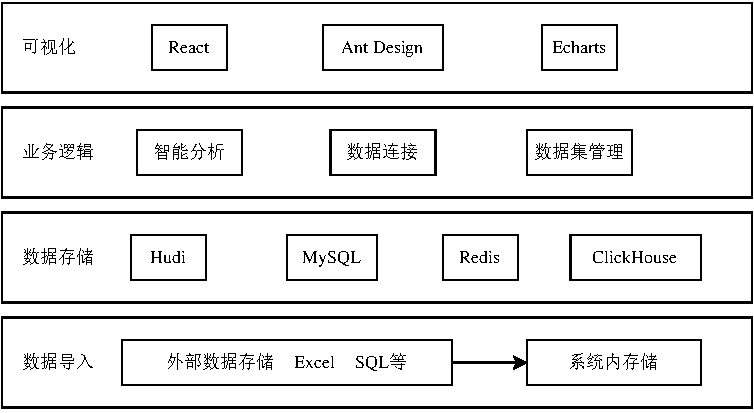
\includegraphics{figure/系统架构图.pdf}
    \label{fig:sysstruc}
\end{figure}
由图中可以看出,系统采用分层的架构设计,这些层相对独立,各自专注于实现自身的功能,而不会直接依赖于其他层次的实现细节。层与层之间通过暴露的接口进行交互,实现数据和控制流的传递。有助于降低系统内部的耦合度,即各个组件之间的依赖关系较弱,提高了系统的灵活性和可维护性。
系统由底向上主要分为数据接入层,数据存储层、业务层和可视化层。下面是各个层的详细介绍。

(1)数据接入层

数据接入层负责将外部的异构数据导入到系统中,其中外部的异构数据源包括数据库数据(关系型数据库如SQL Server、MySQL;非关系型数据库HBase;外部文件数据CSV、XML、JSON等)。这些数据将通过Spark来导入到数据湖Apache Hudi中。
Spark提供了多种接口来对应不同的文件类型数据的导入。

(2)数据存储层

数据存储层主要是对系统中所有数据进行持久化的存储。其中包括大数据存储、业务数据存储和数据缓存。其中大数据存储主要通过数据湖框架Apache Hudi来对原始数据进行持久化存储,前面数据接入层的多源异构数据主要存储在这里。
业务数据主要存储在MySQL中,业务数据主要是针对系统提供服务,保证系统的正常运行。Redis和ClickHouse主要负责数据的缓存,其中Redis缓存的是业务数据,例如用户会话信息、登录状态、用户配置等。clickHouse主要是用于数据分析
过程,进行数据计算和中间结果的存储。

(3)业务层 

业务层负责处理业务逻辑和功能实现。它包含了系统的核心功能模块,通过提供访问接口来解析用户的行为,并将其转化为系统内部的各种调用。在业务层中,不同的功能模块专注于各自的业务规则和业务对象之间的交互,执行完毕后将结果返回给可视化层。业务层采用高内聚、低耦合的系统设计思路,确保各个功能模块之间的独立性和可维护性,同时按照对扩展开放的原则进行设计,以保证整体业务的可扩展性。
业务层具体包含了数据连接、数据管理、智能分析、可视化展示和用户权限几个模块。

(4)可视化层

可视化层是用户与系统的桥梁,用户通过在前端进行操作来完成自己的一系列业务需求。系统使用React作为可视化框架,采用Ant Design作为前端的UI组件库,使用Echarts来创建丰富、交互式的数据可视化图表,并通过Axios和WebSocket来
实现钱后端的通信。

\section{系统业务模块设计与实现}
本节根据前文中提出的系统的业务模块,通过对重要的数据连接、数据管理和智能分析模块的实现类图进行详细的描述,介绍系统业务模块的设计。
\subsection{数据连接模块}
数据连接用于将目标数据源连接到系统中,接入系统中的目标数据源可以在后续的进行数据管理、数据分析等一系列操作。数据连接类型的类图如图\ref{fig:dataconnclass}所示。
% \begin{figure}[H]
%     \centering
%     \caption{数据连接类型管理类图}
%     \includepdf{/Users/latiestqiu/szQshare/SynologyDrive/DRAW/out/class_diagram/class_数据连接/class_数据连接.pdf}
%     \label{fig:dataconnectypelass}
% \end{figure}
当系统用户发起一个请求时,DataConnectionController负责接收这个请求并解
析其中的参数。它随后会调用DataConnectionControllerService中定义的方法来执行具体的操作。DataConnectionControllerServiceImpl类实现了DataConnectionControllerService接口,它包含了系统
的主要业务逻辑。用户访问数据连接页面时,系统会调用 findAllDataConnection()
方法来检索系统中所有已建立的数据连接实例。在这个页面上,用户可以通过执行
establishInstance() 方法来创建一个新的数据连接实例,通过执行 testConnection() 方法
来测试现有数据连接是否正常工作,通过调用 deleteDataConnection() 方法来删除
一个数据连接实例,通过调用 modifyDataConnection() 方法来更新数据连接的信
息,以及通过调用 findDataConnectionInfo() 方法来查看已存在的数据连接配置信
息。DataDataConnection类是数据连接
实例的实体类,存储了平台中数据连接实例的信息,包括连接名称、连接 URL、连接
实例信息(用户名、密码等)等。DataDataConnectionMapper是用于与
数据库中数据连接实例信息表交互的接口。
\subsection{数据管理模块}
数据管理模块主要包括三个部分:目录管理、数据集管理和数据集更新。在目录管理中,主要任务是整理数据集的存储位置,确保它们正确归档在特定文件夹内。目录由不同的节点组成,包括文件夹和数据集本身,它们在目录中以不同的方式标记以便区分。保持这些节点之间的层次结构有助于形成一个有层次的目录结构。

在数据集管理方面,我们可以创建、删除、复制和查看数据集,以便有效地管理它们。

对于数据集更新,它允许数据集按计划或周期性地更新。更新可以是自动的,也可以是手动的。每个数据集都有一个关于如何更新的设置,如果用户未做设置,则使用默认配置。根据这些设置,平台会定期或按需更新数据集,并记录更新任务的详细信息和状态。

更新时,系统确保每个数据集同时只能有一个更新任务在进行。这是通过检查一个特殊的Map实现的,该Map确保每个数据集同时只有一个关联的更新任务正在运行。更新任务的执行是多线程的,使用了一个特定的线程池,该线程池可以调度周期性任务。对于一次性的手动更新,任务会直接提交给线程池执行。
数据管理模块的类图如图\ref{fig:datamanageclass}所示。
\begin{figure}[H]
    \centering
    \caption{数据管理模块类图}
    \label{fig:datamanageclass}
\end{figure}
当前端发出请求时,DataManagementController将充当主要接口来处理并分析这些请求。目录和数据集的管理任务都通过DataSourceService接口完成,而数据集的具体动作则是由DatasetUpdateServiceImpl接口负责。在这种设置下,文件夹和数据集被看作是目录结构的元素,它们虽然共处一个层级,但通过不同的方式标记以区分。
在实现方面,DirectoryServiceImpl和DatasetImpl分别实现了DataSourceService接口的具体职责,处理不同的数据管理需求。当用户进入数据管理页面时,系统首先会调用getTotalCatalog()方法来获得全部资源目录结构。通过makeRootDir()方法可以创建在根目录创建新的文件夹,此外,还可以对文件夹进行移动、删除、重命名等操作。
通过文件夹进入到具体的数据集后,DatasetImpl的previewData()方法会将得到数据集的具体内容,前端通过与controller通信读取内容后经过处理,可以将预览数据集的结果显示在用户界面上。该处还支持用户通过establishDIYDataset()等方法上传自己的数据集、Excel文件、删除数据集等。
在数据模型方面,我们区分了两种类型的信息实体:DirectoryInfo 代表目录节点,而 DatasetInfo 代表数据集节点。DatasetUpdateServiceImpl是对DatasetUpdateService接口的实现,当进入数据集的更新设置页面后,会先调用getDatasetUpdateInfo()方法来查看
数据集已有的更新设置。随后可以通过setDatasetUpdateInfo()或setAllDatasetUpdateInfo()来修改一个或多个数据集的更新设置。修改完更新设置后,可以通过startDatasetUpdateTask()方法来启动一个更新任务,目前系统近支持
全量更新。随后可以关闭更新任务。同时getAllDatasetUpdateInfo()方法也可以查看用户的所有数据集更新信息。
最后,为了实现数据的持久化,系统设计了三个映射类:DirectoryMapper、DatasetMapper 和 DatasetUpdateMapper,它们分别对应于目录管理、数据集管理和数据操作功能,确保所有相关数据都能被持久化存储并管理。
系统的架构遵循Controller-Service-Mapper-Model模式,以上提及的各个类相互配合,一起完成数据连接模块的全部功能。
\subsection{智能分析模块}
智能分析模块主要包括气井分类、产气量预测、开关井推荐。其中气井分类为第三章通过时间序列聚类对气井聚类之后的结果,用于企业对气井的精细化管理。产气量预测为第四章产气量预测的结果,企业可以根据预测结果完成进行
策略制定。开关井推荐也在第四章做过介绍,企业可以根据开关井推荐的结果来进行相应的开关井操作。
智能分析模块的类图如图\ref{fig:analyclass}所示。
\begin{figure}[H]
    \centering
    \caption{智能分析模块类图}
    \label{fig:analyclass}
\end{figure}
由于智能分析多是用Python进行算法实现,实现方式也在前文进行了介绍。因此当前端进入智能分析页面后,IntelligentAnalysisController接口会分析findAllCluster()的参数,然后在IntelligentAnalysisServiceImpl类中调用Python结果,通过WellMapper查询气井信息,最后将结果展示在首页。
产气量预测与开关井推荐等也类似该方法。
\section{系统测试}
\subsection{测试环境说明}
气井智能管控系统的测试环境分为硬件环境和软件环境,表\ref{tab:systesthaen}所示为气井智能管控系统的硬件测试环境.其中硬件环境包括数
据湖底层依赖的Hadoop 集群所需的一个主节点和两个从节点。
% \begin{table}[h]
%     \centering
%     \caption{硬件环境信息表}
%     \label{tab:hardware_info}
%     \begin{tabular}{|l|l|l|l|l|l|}
%     \hline
%     \textbf{机器类型} & \textbf{内存} & \textbf{CPU型号} & \textbf{服务器型号} & \textbf{操作系统} & \textbf{磁盘} \\ \hline
%     Master 主节点   & 64G  & Intel(R) Xeon(R) CPU E5-2683 v3 & 华为 FusionServer 2288H V5 & CentOS7 & 2T \\ \hline
%     slave1 从节点    & 16G  & Intel(R) Xeon(R) E5-2600 v4     & 华为 FusionServer 2288H V5 & CentOS7 & 1T \\ \hline
%     Slave2 从节点    & 16G  & Intel(R) Xeon(R) E5-2600 v4     & 华为 FusionServer 2288H V5 & CentOS7 & 1T \\ \hline
%     \end{tabular}
%     \label{tab:systesthaen}
% \end{table}    
% 表\ref{tab:systestsoen}
% 所示为气井智能管控系统的软件测试环境。
% \begin{table}[h]
%     \centering
%     \caption{软件环境信息表}
%     \label{tab:software_info}
%     \begin{tabular}{|l|l|l|}
%     \hline
%     \textbf{模块名称} & \textbf{软件名称} & \textbf{版本号} \\ \hline
%     操作系统 & CentOS & 7.6 \\ \hline
%     数据库   & MySQL & 7.0 \\ \hline
%     数据缓存   & Redis & 4.0 \\ \hline
%     Hadoop 集群 & Hadoop & 2.7.3 \\ \hline
%     Java 开发   & JDK & 1.8 \\ \hline
%     算法        & Python & 3.9 
%     客户端访问   & Chrome 浏览器 & 88.0.4324.150 \\ \hline
%     \end{tabular}
%     \label{tab:systestsoen}
% \end{table}
\subsection{系统功能性测试}
本小节从系统功能性需求出发,为每个模块设计测试用例和场景并记录结果。

(1)数据连接

数据连接管理模块主要包括新建数据连接、删除数据连接、编辑数据连接和测试
连接四个功能,其测试用例如表\ref{tab:testcon}所示。
\begin{table}[h!]
    \renewcommand{\arraystretch}{1.5}
    \centering
    \begin{tabular}{|c|c|c|c|}
        \hline
        编号 & 用例说明 &  测试步骤 & 预期结果 \\
        \hline
        1 & 创建数据连接 &  选择新建数据连接,输入数据库配置参数,完成数据连接 & 新建数据连接成功 \\
        \hline
        2 & 删除数据连接 & 选择一个数据连接,点击删除按钮 & 删除数据连接成功\\
        \hline
        3 & 编辑数据连接 & 选择一个数据连接,修改其参数配置并提交 & 编辑数据连接成功 \\
        \hline
        4 & 测试数据连接 & 选择一个数据连接,选择测试按钮 & 测试这个数据连接当前是否是成功的 \\
    \end{tabular}
    \caption{用例详细信息}
\end{table}
根据表\ref{tab:testcon}的测试内容,可以在数据连接页面进行创建、删除、编辑和测试连接等操作。





